\chapter{Capitolo 1}


Prova del capitolo 1.

\begin{equation}
    F = ma
\end{equation}


\begin{equation}
    F = ma
\end{equation}


\begin{equation}
    F = ma
\end{equation}


\begin{equation}
    F = ma
\end{equation}



\begin{figure}
    \centering
    \begin{subfigure}[b]{0.15\textwidth}
        \centering
        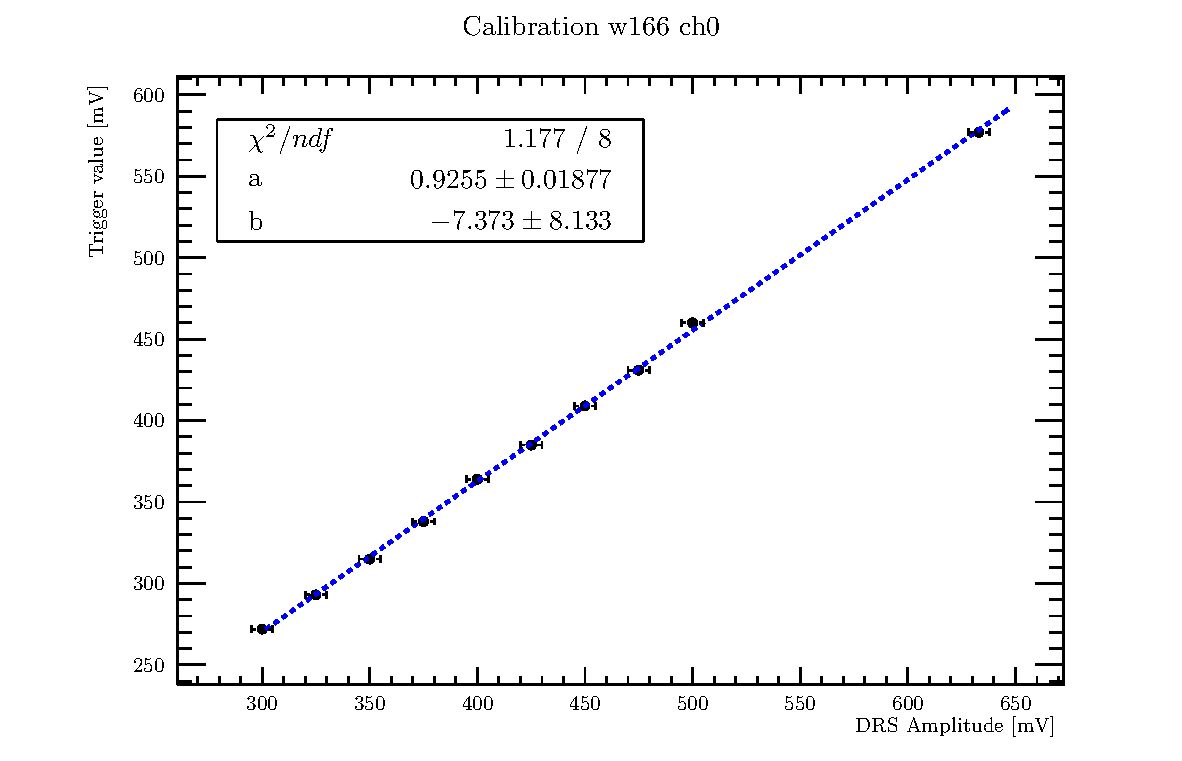
\includegraphics[width=\textwidth]{figures/ch0.pdf}
        \caption{$y=x$}
        \label{fig:y equals x}
    \end{subfigure}
    \hfill
    \begin{subfigure}[b]{0.15\textwidth}
        \centering
        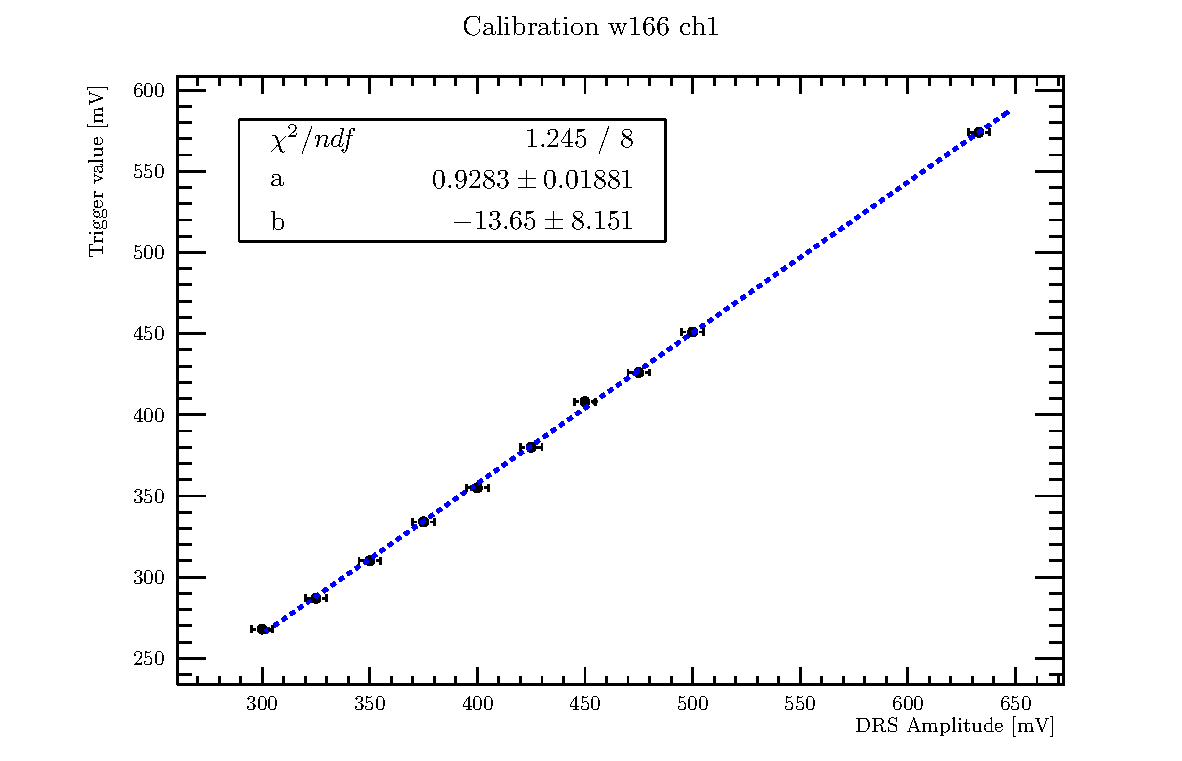
\includegraphics[width=\textwidth]{figures/ch1.pdf}
        \caption{$y=3sinx$}
        \label{fig:three sin x}
    \end{subfigure}
\end{figure}







